%% This is file `cag-template.tex',
%DIF LATEXDIFF DIFFERENCE FILE
%DIF DEL /dir/cag-template_old.tex   Wed Nov 30 23:18:45 2022
%DIF ADD /dir/cag-template.tex       Wed Nov 30 23:18:45 2022
%% 
%% Copyright 2018 Elsevier Ltd
%% 
%% This file is part of the 'Elsarticle Bundle'.
%% ---------------------------------------------
%% 
%% It may be distributed under the conditions of the LaTeX Project Public
%% License, either version 1.2 of this license or (at your option) any
%% later version.  The latest version of this license is in
%%    http://www.latex-project.org/lppl.txt
%% and version 1.2 or later is part of all distributions of LaTeX
%% version 1999/12/01 or later.
%% 
%% The list of all files belonging to the 'Elsarticle Bundle' is
%% given in the file `manifest.txt'.
%% 
%% Template article for Elsevier's document class `elsarticle'
%% with harvard style bibliographic references
%%
%% $Id: cag-template.tex 151 2018-11-22 04:42:39Z rishi $
%%
%% Use the options `twocolumn,final' to obtain the final layout
%% Use `longtitle' option to break abstract to multiple pages if overfull.
%% For Review pdf (With double line spacing)
%\documentclass[times,twocolumn,review]{elsarticle}
%% For abstracts longer than one page.
%\documentclass[times,twocolumn,review,longtitle]{elsarticle}
%% For Review pdf without preprint line
%\documentclass[times,twocolumn,review,nopreprintline]{elsarticle}
%% Final pdf
%\documentclass[times,twocolumn,final]{elsarticle}
%%
\documentclass[times,twocolumn,final]{elsarticle}
%%


%% Stylefile to load CAG template
\usepackage{cag}
\usepackage{framed,multirow}

%% The amssymb package provides various useful mathematical symbols
\usepackage{amssymb}
\usepackage{latexsym}

% Following three lines are needed for this document.
% If you are not loading colors or url, then these are
% not required.
\usepackage{url}
\usepackage{xcolor}
\definecolor{newcolor}{rgb}{.8,.349,.1}

\usepackage{hyperref}

\usepackage[switch,pagewise]{lineno} %Required by command \linenumbers below
\usepackage{booktabs}
\usepackage{overpic}
\usepackage{subfigure}
\usepackage{amsmath}

\journal{Computers \& Graphics}
%DIF PREAMBLE EXTENSION ADDED BY LATEXDIFF
%DIF UNDERLINE PREAMBLE %DIF PREAMBLE
\RequirePackage[normalem]{ulem} %DIF PREAMBLE
\RequirePackage{color}\definecolor{RED}{rgb}{1,0,0}\definecolor{BLUE}{rgb}{0,0,1} %DIF PREAMBLE
\providecommand{\DIFaddtex}[1]{{\protect\color{blue}\uwave{#1}}} %DIF PREAMBLE
\providecommand{\DIFdeltex}[1]{{\protect\color{red}\sout{#1}}}                      %DIF PREAMBLE
%DIF SAFE PREAMBLE %DIF PREAMBLE
\providecommand{\DIFaddbegin}{} %DIF PREAMBLE
\providecommand{\DIFaddend}{} %DIF PREAMBLE
\providecommand{\DIFdelbegin}{} %DIF PREAMBLE
\providecommand{\DIFdelend}{} %DIF PREAMBLE
\providecommand{\DIFmodbegin}{} %DIF PREAMBLE
\providecommand{\DIFmodend}{} %DIF PREAMBLE
%DIF FLOATSAFE PREAMBLE %DIF PREAMBLE
\providecommand{\DIFaddFL}[1]{\DIFadd{#1}} %DIF PREAMBLE
\providecommand{\DIFdelFL}[1]{\DIFdel{#1}} %DIF PREAMBLE
\providecommand{\DIFaddbeginFL}{} %DIF PREAMBLE
\providecommand{\DIFaddendFL}{} %DIF PREAMBLE
\providecommand{\DIFdelbeginFL}{} %DIF PREAMBLE
\providecommand{\DIFdelendFL}{} %DIF PREAMBLE
%DIF HYPERREF PREAMBLE %DIF PREAMBLE
\providecommand{\DIFadd}[1]{\texorpdfstring{\DIFaddtex{#1}}{#1}} %DIF PREAMBLE
\providecommand{\DIFdel}[1]{\texorpdfstring{\DIFdeltex{#1}}{}} %DIF PREAMBLE
%DIF LISTINGS PREAMBLE %DIF PREAMBLE
\RequirePackage{listings} %DIF PREAMBLE
\RequirePackage{color} %DIF PREAMBLE
\lstdefinelanguage{DIFcode}{ %DIF PREAMBLE
%DIF DIFCODE_UNDERLINE %DIF PREAMBLE
  moredelim=[il][\color{red}\sout]{\%DIF\ <\ }, %DIF PREAMBLE
  moredelim=[il][\color{blue}\uwave]{\%DIF\ >\ } %DIF PREAMBLE
} %DIF PREAMBLE
\lstdefinestyle{DIFverbatimstyle}{ %DIF PREAMBLE
	language=DIFcode, %DIF PREAMBLE
	basicstyle=\ttfamily, %DIF PREAMBLE
	columns=fullflexible, %DIF PREAMBLE
	keepspaces=true %DIF PREAMBLE
} %DIF PREAMBLE
\lstnewenvironment{DIFverbatim}{\lstset{style=DIFverbatimstyle}}{} %DIF PREAMBLE
\lstnewenvironment{DIFverbatim*}{\lstset{style=DIFverbatimstyle,showspaces=true}}{} %DIF PREAMBLE
%DIF END PREAMBLE EXTENSION ADDED BY LATEXDIFF

\begin{document}

\verso{Preprint Submitted for review}

\begin{frontmatter}

\title{Anisotropic screen space rendering for particle-based fluid simulation
% \tnoteref{tnote1}
}%
% \tnotetext[tnote1]{Only capitalize first
% word and proper nouns in the title.}

\author{\snm{Anonymous}}
% \author[1]{First Author Given Name \snm{Surname}\corref{cor1}}
% \cortext[cor1]{Corresponding author: 
%   Tel.: +0-000-000-0000;  
%   fax: +0-000-000-0000;}
% \emailauthor{example@email.com}{Corresponding Author Name}
%\ead{example@email.com}

% \author[2]{Second Author Given Name \snm{Surname}\fnref{fn1}}
% \fntext[fn1]{Footnote 1.}  

% \address[1]{Address, City, Postcode, Country}
% \address[2]{Address, City, Postcode, Country}

%\received{1 February 2017}
\received{\today}
%%%% Do not use the below for submitted manuscripts
%\finalform{28 March 2017}
%\accepted{2 April 2017}
%\availableonline{15 May 2017}
%\communicated{S. Sarkar}


\begin{abstract}
%%%
In this paper we propose a real-time fluid rendering method based on the screen space rendering scheme for particle-based fluid simulation. Our method applies anisotropic transformations to the point sprites to stretch the point sprites along appropriate axes, obtaining smooth fluid surfaces based on the weighted principal components analysis of the particle distribution. Then we combine the processed anisotropic point sprite information with popular screen space filters like curvature flow and narrow-range filters to process the depth information. Experiments show that the proposed method can efficiently resolve the issues of jagged edges and unevenness on the surface that existed in previous methods while preserving sharp high-frequency details.
%%%%
\end{abstract}

\begin{keyword}
%% MSC codes here, in the form: \MSC code \sep code
%% or \MSC[2008] code \sep code (2000 is the default)
%\MSC 41A05\sep 41A10\sep 65D05\sep 65D17
%% Keywords
\KWD Real-time rendering\sep Screen space rendering\sep Fluid simulation\sep Smoothed particle hydrodynamics
\end{keyword}

\end{frontmatter}

\linenumbers

%% main text
\section{Introduction}
\label{sec1}
The physics-based fluid simulation has great application value in the fields of both Computer-aided Engineering (CAE) and Computer Graphics (CG).
Among all the simulation methods, the \emph{particle-based} approaches like \emph{Smoothed Particle Hydrodynamics} (SPH) have received much attention for their algorithmic efficiency and application flexibility~\cite{Ihmsen14}. 
However, for the visualization of particle-based simulation results, tracing surfaces for particle-represented fluid has been the computation bottleneck of the whole process. Hence, how to efficiently visualize the simulated fluid while maintaining proper fidelity has become a hot research topic.

Instead of directly tracing the particle surface and constructing the polygon mesh, the \emph{screen space rendering} approach avoids these expensive processes by only generating surface with respect to the camera using the depth and thickness information. In this way, particles are handled as \emph{point sprites}, 2D textures facing the camera (usually in a round shape). The edges between textures are smoothed out to produce fluid surface effects for the screen\cite{ref:ref2}. This approach avoids the expensive mesh construction procedure, making real-time fluid simulation viable for gaming and state-of-the-art virtual reality applications\cite{ref:ref3}. 

But several inherited artefacts of screen space rendering hinder its further exploitation and integration into a wider range of applications. For example, despite subsequent improvements in the original method, surfaces extracted from particles tend to be uneven, and are often too blurred to make a distinction between the foreground and the background. Inspired by Yu and Turk~\cite{yu2013reconstructing}, we propose an anisotropic transformation scheme for point texture, which is applied before filtering the depth image, to generate smooth surfaces in discontinuous regions and at the same time preserve vivid details.

\section{Related work}
Physics based fluid simulation approaches can be mainly divided into two categories: Eulerian methods~\cite{ref:ref4} which utilize a background grid to discretize space into cells, and meshless Lagrangian methods~\cite{ref:ref7} using particles to represent fluid volumes. For video games, virtual reality, and other real-time graphics applications, particle-based simulation such as SPH~\cite{IISPH2013,DFSPH2015,ref:ref5} is often the more preferred approach due to its high efficiency and flexibility~\cite{carensac2022optimizations}. 

To visualize the Lagrangian simulation results, traditionally, fluid surfaces are first traced and constructed as polygon meshes using the marching cubes algorithm~\cite{ref:ref12,ref:ref6,yang2020completely}. Meshes are then rendered as fluid. The major drawback of this two-step scheme is that the mesh generation process consumes large computational resources and can be quite time-consuming for very detailed results. Some researchers have improved the marching cubes algorithm to achieve real-time mapping with a very small number of particles, but its quality is still unsatisfactory\cite{ref:ref10}.

The screen space rendering technique is an alternative approach for visualizing fluid surfaces. M{\"u}ller et al.\cite{ref:ref2} first applied this method for fluid rendering. It directly draws the fluid surfaces without the need of producing surface mesh, sacrificing fidelity for efficiency. The key factor in determining the rendering result is the choice of smoothing filter. As is shown in Fig.~\ref{fig:figure2}, the jagged depth information derived from fluid particles needs to be firstly smoothed to get the fluid surface. 

A simple Gaussian filter for surface smoothing\cite{ref:ref2} tends to produce unwanted blur effects and is often not ideal. The bilateral Gaussian filter~\DIFdelbegin \DIFdel{\mbox{%DIFAUXCMD
\cite{ref:ref15,neto2017real} }\hspace{0pt}%DIFAUXCMD
}\DIFdelend \DIFaddbegin \DIFadd{\mbox{%DIFAUXCMD
\cite{ref:ref3,neto2017real} }\hspace{0pt}%DIFAUXCMD
}\DIFaddend preserves sharp fluid boundaries, but leads to excessive flattening of discontinuous regions. In addition, the bilateral Gaussian filter is not separable, and an approximate separation can result in visual artefacts. Troung and Yuksek~\cite{truong2018narrow} introduced a narrow-range filtering technique that smooths the depth map by directly using a narrow range of depth values. This method provides improved surface quality in terms of surface smoothness and preserving boundaries near discontinuities.
Recently, Oliveira and Paiva~\cite{oliveira2022narrow} solved the particle deficiency problem~\cite{truong2018narrow} by performing a particle classification mechanism. Liu et al.~\cite{liu2022real} proposed a low-cost differentiable screen-space rendering algorithm for augmented reality (AR).

However, we find that the unevenness of fluid surfaces caused by the distribution of particles has not yet been handled properly in screen space rendering. Inspired by work from Yu and Turk~\cite{yu2013reconstructing}, we provide anisotropic transformation for particle textures prior to the derivation of depth image to get a smoother fluid surface.

\begin{figure}[!t]
    %DIF >  \setlength{\abovecaptionskip}{1mm}
    %DIF >  \setlength{\belowcaptionskip}{-5mm}
    \centering
    \DIFdelbeginFL %DIFDELCMD < \begin{overpic}
%DIFDELCMD <     [%%%
\DIFdelFL{width=}%DIFDELCMD < \linewidth]{%%%
\DIFdelFL{figs/surface_processing.png}%DIFDELCMD < }
%DIFDELCMD <     \put(50,88) %%%
\DIFdelendFL \DIFaddbeginFL \subfigure[isotropic] \DIFaddendFL {
    \DIFdelbeginFL \DIFdelFL{camera}\DIFdelendFL \DIFaddbeginFL 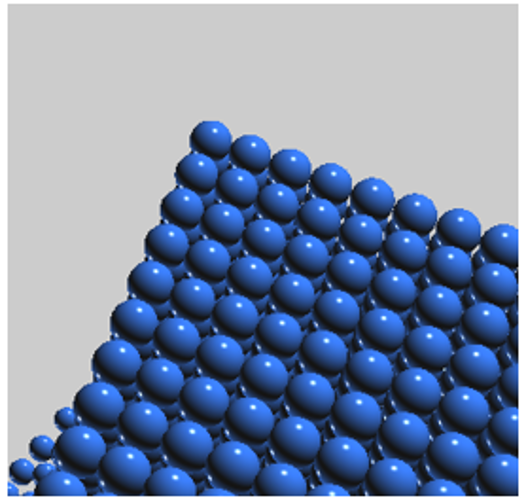
\includegraphics[width=0.47\linewidth]{figs/isotropic.png}
    \DIFaddendFL }    
    \DIFdelbeginFL %DIFDELCMD < \put(55,63) %%%
\DIFdelendFL \DIFaddbeginFL \subfigure[anisotropic] \DIFaddendFL {
    \DIFdelbeginFL \DIFdelFL{foreground surface}\DIFdelendFL \DIFaddbeginFL 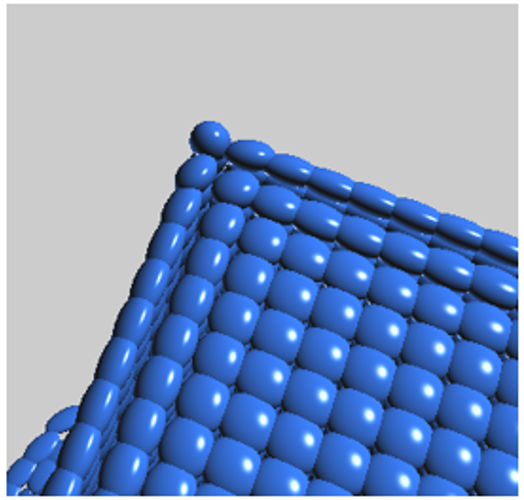
\includegraphics[width=0.47\linewidth]{figs/anisotropic.png}
    \DIFaddendFL } 
    \DIFdelbeginFL %DIFDELCMD < \put(5,37) %%%
\DIFdelendFL \DIFaddbeginFL \caption{\DIFaddFL{Comparison of isotropic and anisotropic fluid particles.}}
    \label{fig:figure3}
\end{figure}

\begin{figure}[!t]
    %DIF >  \setlength{\abovecaptionskip}{1mm}
    %DIF >  \setlength{\belowcaptionskip}{-5mm}
    \centering
    \subfigure[isotropic] \DIFaddendFL {
    \DIFdelbeginFL \DIFdelFL{background surface}\DIFdelendFL \DIFaddbeginFL 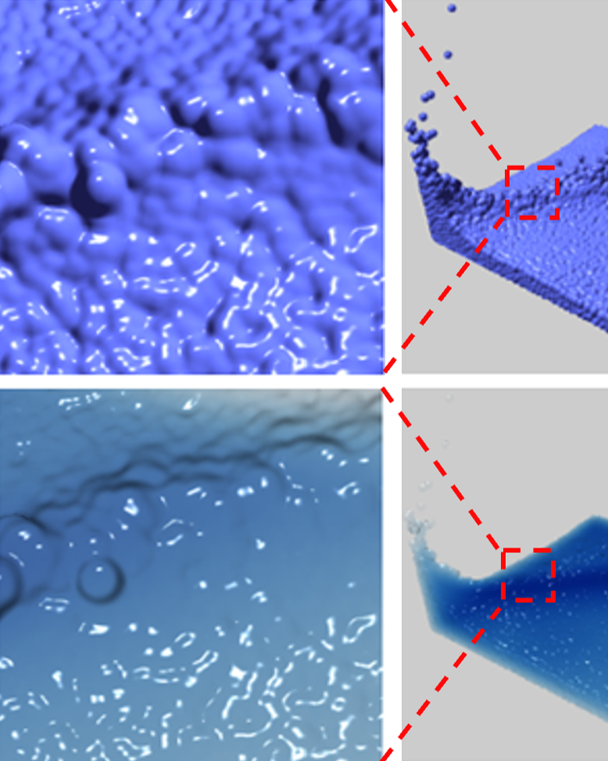
\includegraphics[width=0.22\textwidth]{figs/figure5_1_new.png}
    \DIFaddendFL }    
    \DIFdelbeginFL %DIFDELCMD < \put(63,5) %%%
\DIFdelendFL \DIFaddbeginFL \subfigure[anisotropic] \DIFaddendFL {
    \DIFdelbeginFL \DIFdelFL{refraction direction}\DIFdelendFL \DIFaddbeginFL 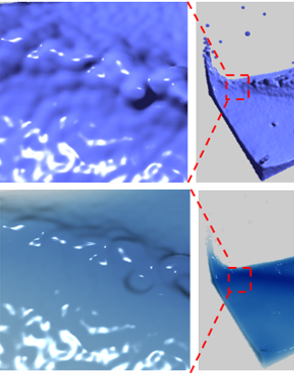
\includegraphics[width=0.22\textwidth]{figs/figure5_2_new.png}
    \DIFaddendFL } 
    \DIFdelbeginFL %DIFDELCMD < \end{overpic}
%DIFDELCMD < %%%
\DIFdelendFL \caption{\DIFdelbeginFL \DIFdelFL{The schematic diagram }\DIFdelendFL \DIFaddbeginFL \DIFaddFL{Experimental comparison }\DIFaddendFL of \DIFdelbeginFL \DIFdelFL{surface processing }\DIFdelendFL \DIFaddbeginFL \DIFaddFL{isotropy and anisotropy }\DIFaddendFL in \DIFdelbeginFL \DIFdelFL{screen space rendering method}\DIFdelendFL \DIFaddbeginFL \DIFaddFL{the dam break scenario}\DIFaddendFL .}
    \DIFdelbeginFL %DIFDELCMD < \label{fig:figure1}
%DIFDELCMD < %%%
\DIFdelendFL \DIFaddbeginFL \label{fig:figure4}
\DIFaddendFL \end{figure}

\section{Real-time Screen Space Fluid Rendering}
Fluid rendering in the screen space is performed by drawing the 3D fluid directly into the 2D screen without generating surface meshes, as shown in Fig.\ref{fig:figure1}, and is closely related to image processing algorithms~\DIFdelbegin \DIFdel{\mbox{%DIFAUXCMD
\cite{ref:green2010screen}}\hspace{0pt}%DIFAUXCMD
}\DIFdelend \DIFaddbegin \DIFadd{\mbox{%DIFAUXCMD
\cite{ref:ref3}}\hspace{0pt}%DIFAUXCMD
}\DIFaddend . The schematic diagram describing the procedure of the surface rendering algorithm is shown in Fig.\ref{fig:figure2} and is detailed in the following.

\subsection{Depth Information}

\paragraph{Deriving the Depth Information}
First, the distance $z_i$ between each particle and camera pixel $i$ is calculated from the camera viewpoint~\cite{ref:ref20}.
To obtain the fluid surface from the camera point of view, the point sprite~\cite{ref:ref21} method is used to render the particles as spheres, which allows us to directly extract the depth values from the video memory buffer.

\paragraph{Smoothing Depth Information}
Direct use of spherical point sprites as depth information usually produces uneven fluid surfaces. To reduce the rugged effects, specific filters are applied to the depth image, flattening the abrupt bumps of particles by averaging $z_i$ for local pixels. One of the most common smoothing filters is a Gaussian filter\cite{ref:ref24}, with the formula:
\begin{equation}
    G\left({\mathbf{p}}_i, {\mathbf{p}}_j, \sigma_i\right)
    =
    \frac{1}{2 \pi \sigma_i^{2}} e^{-\frac{ \| {\mathbf{p}}_i - {\mathbf{p}}_j \| }{2 \sigma_i^{2}}} , 
\label{con:equ2}
\end{equation}

where $j$ is the neighbour pixel of $i$, $\sigma$ is the standard deviation parameter determined by $z_i$~\cite{truong2018narrow}, and ${\mathbf{p}}$ describes the location for each pixel in the screen space. 
The Gaussian convolution can obtain smooth particle depth information. However, it can cause over-smoothing, leading to some loss of edges. Therefore, variants such as the bilateral Gaussian method are often used to obtain better results.

\begin{figure*}[!t]
\centering
\DIFdelbeginFL %DIFDELCMD < 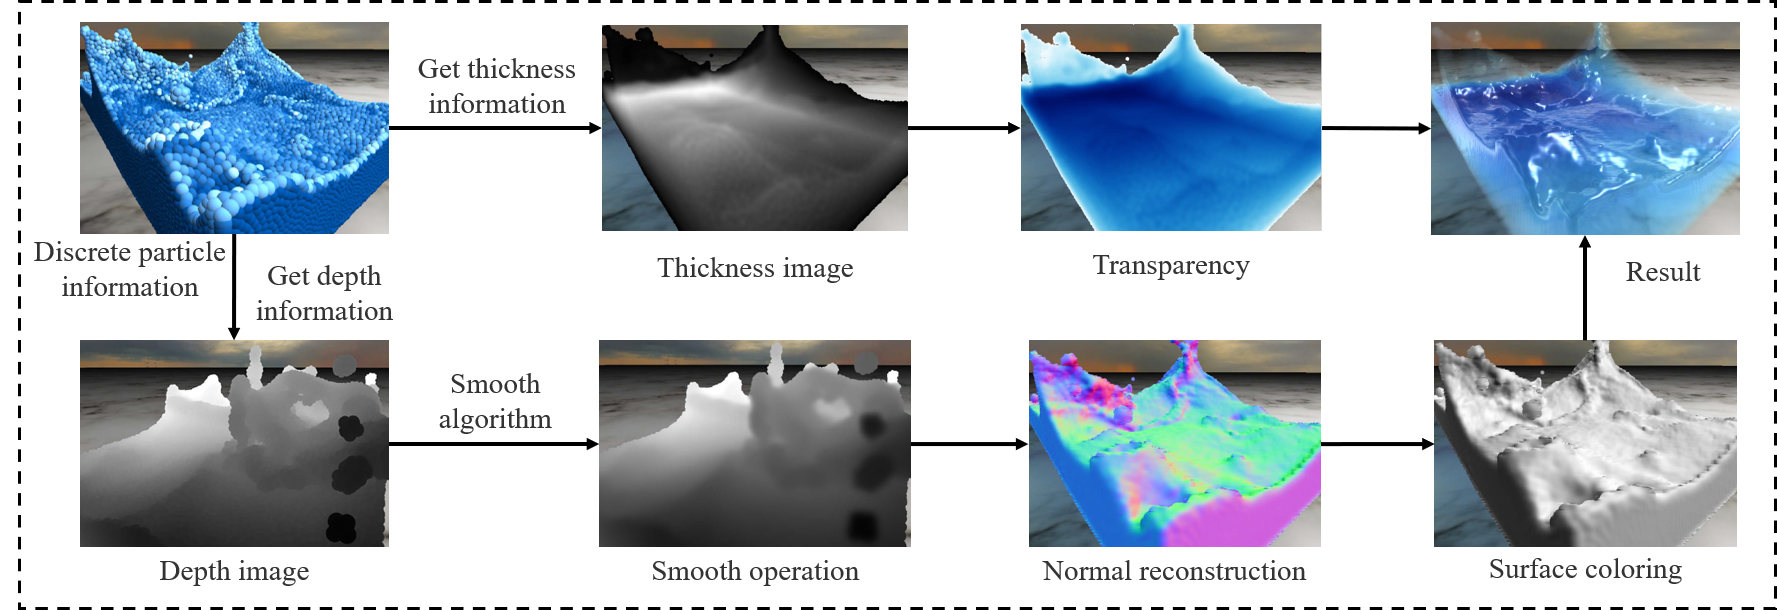
\includegraphics[scale=.6]{figs/figure2_b.png}
%DIFDELCMD < %%%
\DIFdelendFL \DIFaddbeginFL 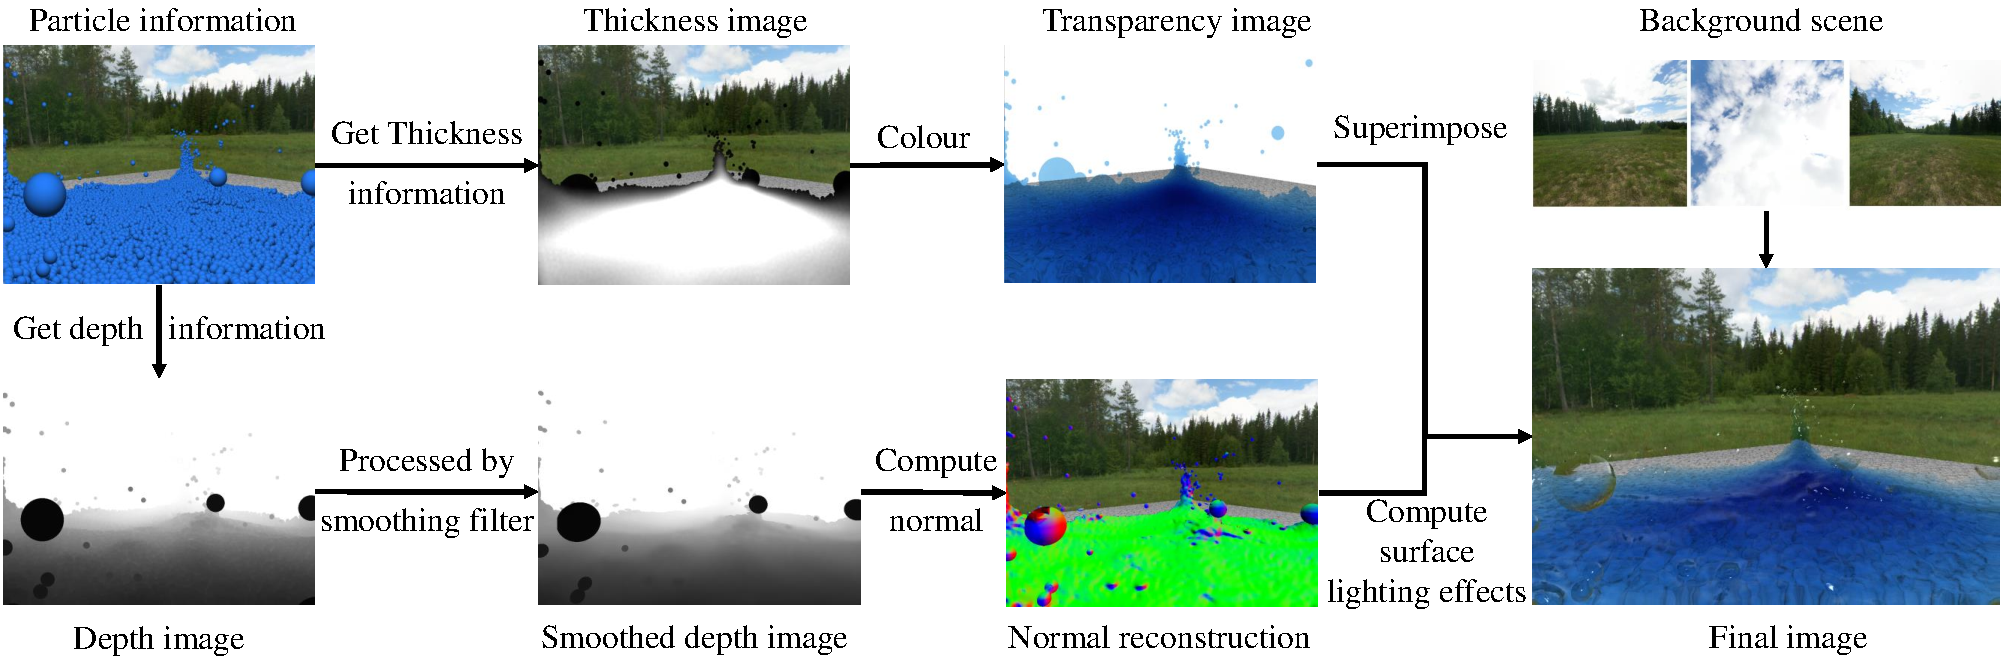
\includegraphics[width=\linewidth]{figs/figure2_b.pdf}
\DIFaddendFL \caption{Schematic flow diagram of \DIFdelbeginFL \DIFdelFL{our algorithm}\DIFdelendFL \DIFaddbeginFL \DIFaddFL{screen space rendering pipeline for fluid rendering}\DIFaddendFL : First, transform the fluid particles to the screen space and obtain the depth information and thickness information. Second, post-process the depth image, reconstruct normal on the depth image and render the fluid surface using normal and thickness information.}
\label{fig:figure2}
\end{figure*}

\subsection{Thickness Information}
Fluid distribution in the real world is not uniform, so it is necessary to calculate the amount of fluid between the camera and the nearest opaque object, which is called the thickness image. When shading, the thickness image is used to calculate the colour and transparency of the fluid\cite{ref:ref14}. The formula is given as:
\begin{equation}
    T(\mathbf{{p}}_i)=\sum_{j=0}^{n} G\left( \| \mathbf{{p}}_i - \mathbf{\hat{x}}_j \| \right), 
\label{con:equa3}
\end{equation}
where $n$ represents all fluid particles, $\mathbf{\hat{x}}_j$ corresponds to the projection position of particle $\mathbf{{x}}_j$ in the screen space. This calculation is correct when the particles do not overlap. Because of the incompressibility of the SPH method (particles seldom overlap), the thickness information can be calculated by Eqn.~\ref{con:equa3}.

\DIFaddbegin \begin{figure}[!t]
\centering
\begin{overpic}
    [\DIFaddFL{width=}\linewidth]{\DIFaddFL{figs/surface_processing.png}}
    \put(50,88) {\DIFaddFL{camera}}
    \put(55,63) {\DIFaddFL{foreground surface}}
    \put(5,37) {\DIFaddFL{background surface}}
    \put(63,5) {\DIFaddFL{refraction direction}}
\end{overpic}
\caption{\DIFaddFL{The schematic diagram of surface processing in screen space rendering method.}}
\label{fig:figure1}
\end{figure}

\DIFaddend \subsection{Normal Reconstruction and Surface Shading}
After obtaining the vertex coordinates in camera space, the normal needs to be reconstructed from the coordinates to handle light reflection and refraction on the surface. The partial derivatives are calculated according to the finite difference method.

Afterwards, the refraction of the fluid~\cite{ref:ref25} and Blinn-Phong illumination~\cite{ref:ref27} are calculated. The relationship between the transmittance of the fluid and the thickness of the fluid is obtained according to the Beer-Lambert algorithm\cite{ref:ref28} $I(d)=I_{0} d^{-k d}$, where $d$ is the thickness of the fluid, $I_0$ is the value of light intensity and $k$ is the attenuation coefficient vector of the fluid. Then the final fluid colouring result is obtained.

\section{Anisotropic Transformation of Point Sprites for Fluid Particles}
\subsection{Tracing Surface Using Smoothing Kernel}
In fluid simulation, a finer-grained spatial discretization can be achieved by increasing the simulation resolution via representing fluid using smaller particles, which generates smoother edges when being rendered. However, increasing the resolution for 3D fluid simulation requires complex computations, which seriously affects the performance in real time. To combine both efficiency and quality, our approach is based on the weighted principal components analysis (WPCA) of SPH fluid particles. We obtain anisotropic kernel functions to obtain anisotropic fluid particles based on their distribution, and use the eigenvalue magnitudes on the eigenvectors as the basis for fluid particle deformation to achieve efficient smoothing and detail preservation.

In particle-based fluid simulation, fluid particles are represented as spheres, which are then used to perform screen space projection based on point sprites or surface reconstruction using the marching cubes algorithm. Since the discrete fluid particles are isotropic, for a fluid particle $i$ whose centre is located at the spatial coordinate $\mathbf{x}_i$, the approximated value $\phi_i$ of the colour field at its location can be averaged and weighted by all its neighbouring particles as:
\begin{equation}
\phi_{i}=\sum_{j} \frac{m_{j}}{\rho_{j}} W\left(\|\mathbf{x}_i-\mathbf{x}_j\|, h\right),
\label{con:equa9}
\end{equation}
where $m_j$ and $\rho_j$ are the volume and density of the neighbouring fluid particle $j$, $W$ is called the smoothing kernel or kernel function, which is a normalized Gaussian-like function~\cite{Ihmsen14}, $h$ is the support radius of the kernel function, beyond which $W$ takes the value of 0. In this paper, we use an anisotropic smoothing kernel $W(\mathbf{r},\mathbf{B})$ to replace the isotropic function $W(r,h)$ by introducing the anisotropy matrix $\mathbf{B}$ into the kernel function:
\DIFdelbegin %DIFDELCMD < \begin{figure}[!t]
%DIFDELCMD <     %%%
%DIF <  \setlength{\abovecaptionskip}{1mm}
    %DIF <  \setlength{\belowcaptionskip}{-5mm}
    %DIFDELCMD < \centering
%DIFDELCMD <     \subfigure[isotropic] {
%DIFDELCMD <     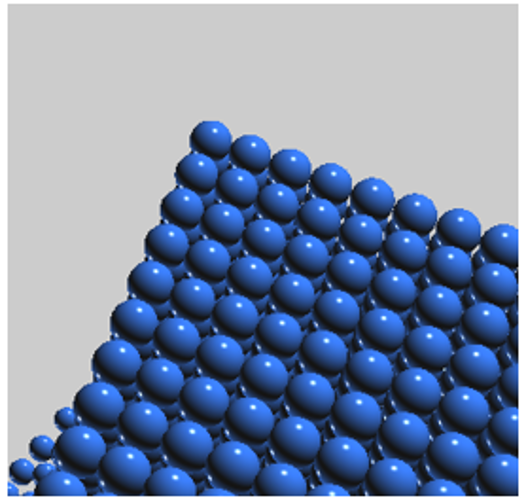
\includegraphics[width=0.47\linewidth]{figs/isotropic.png}
%DIFDELCMD <     }    
%DIFDELCMD <     \subfigure[anisotropic] {
%DIFDELCMD <     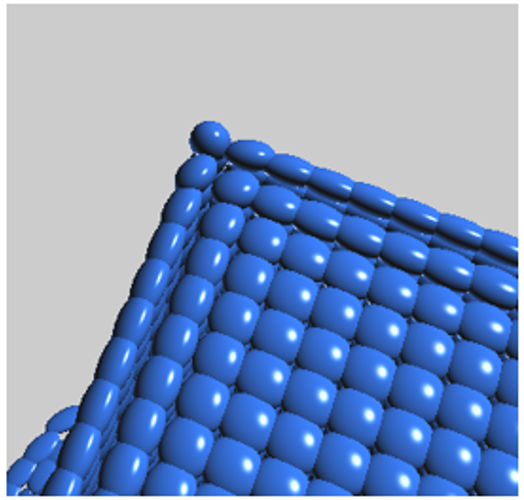
\includegraphics[width=0.47\linewidth]{figs/anisotropic.png}
%DIFDELCMD <     } 
%DIFDELCMD <     %%%
%DIFDELCMD < \caption{%
{%DIFAUXCMD
\DIFdelFL{Comparison of isotropic and anisotropic fluid particles.}}
    %DIFAUXCMD
%DIFDELCMD < \label{fig:figure3}
%DIFDELCMD < \end{figure}
%DIFDELCMD < 

%DIFDELCMD < \begin{figure*}[!t]
%DIFDELCMD <     %%%
%DIF <  \setlength{\abovecaptionskip}{1mm}
    %DIF <  \setlength{\belowcaptionskip}{-5mm}
    %DIFDELCMD < \centering
%DIFDELCMD <     \subfigure[isotropic] {
%DIFDELCMD <     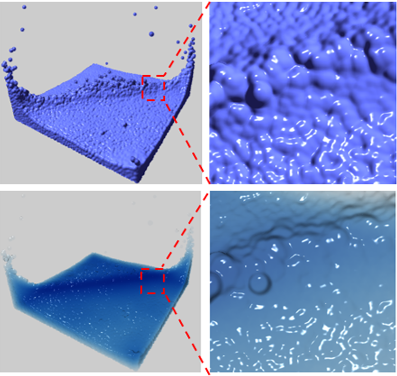
\includegraphics[width=0.48\textwidth]{figs/figure5_1.png}
%DIFDELCMD <     }    
%DIFDELCMD <     \subfigure[anisotropic] {
%DIFDELCMD <     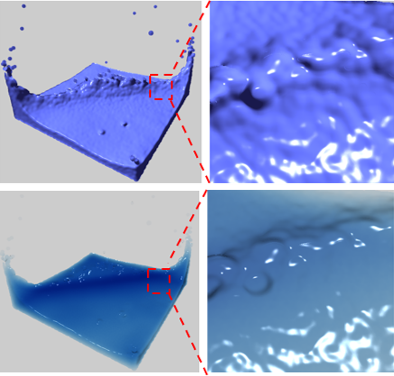
\includegraphics[width=0.48\textwidth]{figs/figure5_2.png}
%DIFDELCMD <     } 
%DIFDELCMD <     %%%
%DIFDELCMD < \caption{%
{%DIFAUXCMD
\DIFdelFL{Experimental comparison of isotropy and anisotropy in the dam break scenario.}}
    %DIFAUXCMD
%DIFDELCMD < \label{fig:figure4}
%DIFDELCMD < \end{figure*}
%DIFDELCMD < %%%
\DIFdelend 


\begin{equation}
W(\mathbf{r},\mathbf{B})=\beta \operatorname{det}(\mathbf{B}) P(|\mathbf{r}\mathbf{B}|),
\label{con:equa10}
\end{equation}
where $\beta$ is the scaling factor, $P$ is a symmetric decaying spline with finite support.

The anisotropy matrix $\mathbf{B}$ makes the smoothing kernel anisotropic by stretching and rotating the relative position $\mathbf{r}$ between particles. Fig.\ref{fig:figure3}(a) shows the fluid particles in normal state, and Fig.\ref{fig:figure3}(b) shows the fluid particles after anisotropic processing. It can be easily observed that particles become more compact and smooth at the edges of the fluid when using the anisotropic representation.

\subsection{Deriving Anisotropy Matrix}
The anisotropic kernel function mentioned above can be considered as a generalization of the isotropic kernel function. Let $\mathbf{I}$ be a d-dimensional unit matrix. When $B=\frac 1 h \mathbf{I}$, $W(\mathbf{r},\mathbf{B})$ returns to $W(r,h)$. To make the values of the kernel function larger along the tangential direction of the fluid surface than the normal direction, or to stretch the kernel along the edges of the fluid, WPCA\cite{ref:ref30} is performed to find the eigenvalues and eigenvectors according to neighbouring fluid particles. Since the Lagrangian simulation algorithm is naturally non-uniform in particle distribution, the use of WPCA method effectively avoids the sensitivity to outliers in the traditional principal component analysis (PCA) method, and enhances the efficiency of surface smoothing.

First, a weight value $\omega_{ij}$ is determined for each pair of fluid particles. A weighted covariance matrix is then constructed using the weight values, and singular value decomposition (SVD) is performed on the covariance matrix. The obtained matrix principal axes as well as the eigenvalues are finally used to construct the anisotropy matrix $\mathbf{B}$. The weighted average position of the fluid is given as $\bar{\mathbf{x}}_{i}=\sum_{j} \omega_{ij} \mathbf{x}_{j}$, where $\omega_{ij}$ is the weight of the fluid neighbor particle $j$ to particle $i$. In this paper we 
compute $\omega_{i j}$ as:

\begin{equation}
\omega_{i j}=\frac{W\left(\left|\mathbf{x}_{i}-\mathbf{x}_{j}\right|, h\right)}{\sum_{j} W\left(\left|\mathbf{x}_{i}-\mathbf{x}_{j}\right|, h\right)}.\label{con:equa11}
\end{equation}

This results in a normalized weighting that is larger when the particles are closer. The displacement of the weighted average position from the original position can indicate the distribution trend of the fluid surface. Based on this trend, a covariance matrix $\mathbf{C}_i$ can be constructed for the fluid particle $i$ as:

\begin{equation}
C_{i}=\sum_{j} \omega_{i j}\left(\mathbf{x}_{j}-\bar{\mathbf{x}}_{i}\right)\left(\mathbf{x}_{j}-\bar{\mathbf{x}}_{i}\right)^{T}\label{con:equa12}.
\end{equation}

A singular value decomposition for the covariance matrix yields $\mathbf{C}_{i}=\mathbf{W} \mathbf{\Sigma} \mathbf{W}^{T}$, where the diagonal matrix $\mathbf{\Sigma} = diag(\sigma_1,\sigma_2,...,\sigma_d)$ contains all the eigenvalues from the largest to the smallest. To obtain a stable anisotropic deformation effect, the minimum of eigenvalues is restricted to a threshold with respect to the largest eigenvalue. The value of $\sigma_k^r$ is chosen as $\sigma_k^r=max(\sigma_1/\kappa,\sigma_k)$ to adjust the smaller eigenvalues so that the ratio of the largest eigenvalue to the smallest one is limited. In our experiments, we choose $\kappa=4$. Furthermore, no anisotropic kernel function is used when the number of neighbouring particles is less than or equal to $20$, and a scale control factor $s$ makes $|s \mathbf{C}| \approx 1$ to keep the particle volume from changing significantly. We select $s=1400$ in our experiments. The regularized covariance matrix can be expressed as:
\begin{equation}
\mathbf{C}^{r}=W \mathbf{\Sigma}^{r} W^{T}.
\end{equation}

\section{Results and Analysis}

\begin{figure}[!t]
    \centering
    \subfigure[isotropic] {
    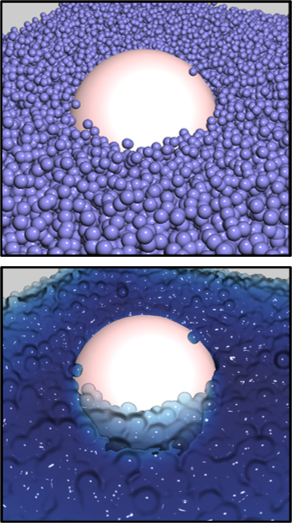
\includegraphics[width=0.46\linewidth]{figs/figure6_4.png}
    }    
    \subfigure[anisotropic] {
    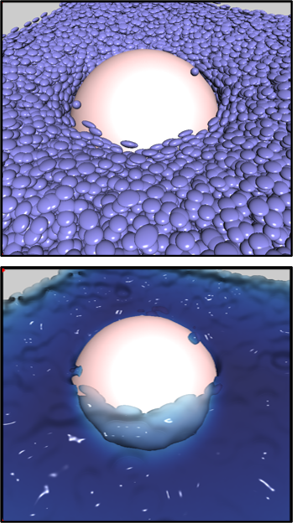
\includegraphics[width=0.46\linewidth]{figs/figure6_5.png}
    } 
    \caption{Experimental comparison of isotropy and anisotropy in the fluid-soild coupling scenario.}
    \label{fig:figure5}
\end{figure}

\begin{figure*}[!t]
    \centering
    \DIFdelbeginFL %DIFDELCMD < \subfigure[\vspace{2mm}isotropic point sprites representation]{
%DIFDELCMD <     \begin{overpic}
%DIFDELCMD <     [width=0.48\textwidth]{figs/ball_iso.png}
%DIFDELCMD <     \put(5,2)       {\footnotesize No filter}
%DIFDELCMD <     \put(25,2)      {\footnotesize Gaussian}
%DIFDELCMD <     \put(44,4)      {\footnotesize Curvature}
%DIFDELCMD <     \put(47,0)      {\footnotesize Flow}
%DIFDELCMD <     \put(65,4)      {\footnotesize Bilateral}
%DIFDELCMD <     \put(64.5,0)    {\footnotesize Gaussian}
%DIFDELCMD <     \put(80,2)      {\footnotesize Narrow-Range}
%DIFDELCMD <     \end{overpic}
%DIFDELCMD <     \label{fig:ball_iso}
%DIFDELCMD <     }   
%DIFDELCMD <     \subfigure[anisotropic point sprites representation]{
%DIFDELCMD <     \begin{overpic}
%DIFDELCMD <     [width=0.48\textwidth]{figs/ball_aniso.png}
%DIFDELCMD <     \put(5,2)       {\footnotesize No filter}
%DIFDELCMD <     \put(25,2)      {\footnotesize Gaussian}
%DIFDELCMD <     \put(44,4)      {\footnotesize Curvature}
%DIFDELCMD <     \put(47,0)      {\footnotesize Flow}
%DIFDELCMD <     \put(65,4)      {\footnotesize Bilateral}
%DIFDELCMD <     \put(64.5,0)    {\footnotesize Gaussian}
%DIFDELCMD <     \put(80,2)      {\footnotesize Narrow-Range}
%DIFDELCMD <     \end{overpic}
%DIFDELCMD <     \label{fig:ball_aniso}
%DIFDELCMD <     } 
%DIFDELCMD <     %%%
\DIFdelendFL \DIFaddbeginFL \subfigure[\vspace{2mm}isotropic point sprites representation]{
    \begin{overpic}
    [width=0.48\textwidth]{figs/ball_iso_new.png}
    \put(5,2)       {\footnotesize No filter}
    \put(25,2)      {\footnotesize Gaussian}
    \put(44,4)      {\footnotesize Curvature}
    \put(47,0)      {\footnotesize Flow}
    \put(65,4)      {\footnotesize Bilateral}
    \put(64.5,0)    {\footnotesize Gaussian}
    \put(80,2)      {\footnotesize Narrow-Range}
    \end{overpic}
    \label{fig:ball_iso}
    }   
    \subfigure[anisotropic point sprites representation]{
    \begin{overpic}
    [width=0.48\textwidth]{figs/ball_aniso_new.png}
    \put(5,2)       {\footnotesize No filter}
    \put(25,2)      {\footnotesize Gaussian}
    \put(44,4)      {\footnotesize Curvature}
    \put(47,0)      {\footnotesize Flow}
    \put(65,4)      {\footnotesize Bilateral}
    \put(64.5,0)    {\footnotesize Gaussian}
    \put(80,2)      {\footnotesize Narrow-Range}
    \end{overpic}
    \label{fig:ball_aniso}
    } 
    \DIFaddendFL \caption{Experimental comparison of isotropy and anisotropy in the dam break scenario. Columns 1-5 is the (a) part of this figure, demonstrating surface constructed without anisotropic transformation; Columns 6-10 is the (b) part of this figure, showing how anisotropic transformation works with and without different smoothing filters.}
    \label{fig:ball_iso&aniso}
\end{figure*}

The experiments below are performed using a hardware platform of AMD Ryzen 7 5800H @3.20 GHz, 32GB memory, and NVIDIA RTX 3060. The 3D graphics API OpenGL is used for particle rendering, and C++ is used as the hardware graphics interactive language to process logical operations. In addition, GLSL colouring language is used to calculate the fluid optical effect in GPU. The real-time performance of fluid is maintained during all experiments.

\subsection{Anisotropic Processing Results}
In this subsection, the anisotropic algorithm is adopted to process fluid particles to reduce the roughness of the fluid depth-map, which can improve the final rendering effect of the fluid surface. As shown in Fig.\ref{fig:figure4}, (a) and (b) respectively represent the surface rendering results when two water blocks collide under isotropic and anisotropic conditions. It can be observed that the overall surface rendering results processed by the anisotropic algorithm are smoother, and the illumination shading is more realistic with fine highlights.

In addition, experimental verification is conducted for a fluid-solid coupling scenario, as shown in Fig.~\ref{fig:figure5}. In the fluid-solid coupling scenario, real-time fluid rendering based on the anisotropic algorithm shows better surface results with smoother surfaces, especially at the interface between the rigid body and liquid.

\begin{figure}[!t]
    \centering
    \begin{overpic}
        [width=\linewidth]{figs/figure9.png}
        \put(6,-2)      {\footnotesize Gaussian}
        \put(25,-2)      {\footnotesize Bilateral Gaussian}
        \put(53,-2)      {\footnotesize Curvature Flow}
        \put(78,-2)      {\footnotesize Narrow-Range}
    \end{overpic}
    \caption{From left to right are Gaussian filter, bilateral Gaussian filter, curvature flow filter and narrow-range filter. 
    % All methods use the same number of iterations ($iter = 2$) except the curvature flow-based method with a larger number ($iter = 80$).
    }
    \label{fig:figure6}
\end{figure}

\subsection{Combination with Popular Smoothing Filters}
In this subsection, the anisotropic algorithm is combined with various popular smoothing filters to verify the effectiveness and practicability of the proposed scheme under actual application scenarios. The Gaussian filter, the bilateral Gaussian filter and the narrow-range filter use the same number of iterations ($iter=2$). The curvature flow filter uses more iterations ($iter=80$) to obtain flat surface results, at the cost of performance loss.

% obtain the final fluid rendering effect, and the performance of different filters is compared. The Gaussian filter, the bilateral Gaussian filter and the narrow-range filter use the same number of iterations. The curvature flow filter uses more iterations to obtain flat surface results, at the cost of performance loss.

Fig.~\ref{fig:ball_iso&aniso} demonstrates the scenario where a dam-break fluid collides with multiple differently shaped solid objects. Complex boundary geometries can be observed in this case. Fig.~\ref{fig:ball_iso} and Fig.~\ref{fig:ball_aniso} shows the surfaces constructed using isotropic and anisotropic point sprites respectively. It can be seen that the proposed anisotropic transformation scheme can enhance surface performance with almost every state-of-the-art smoothing filter. The second and the third row of Fig.~\ref{fig:ball_iso&aniso} exhibit how anisotropic transformation reduces the unevenness of particle distribution on the free surface and coupling boundaries. And the fourth row shows our method can also help to gather the sparsely distributed fluid particles representing splashes into more well-organized structures.

Fig.~\ref{fig:figure6} is another experiment that further shows the anisotropic surface generation effects of the fluid under different filters with a more complex fluid-rigid coupling boundary. The Gaussian filter is a separable filter with high computational efficiency. However, it still produces a large amount of noise on the surface, which is far from the desired ideal result. Meanwhile, the boundary morphed into particles due to a lack of neighbouring particles in the splashing area (second row of Fig.~\ref{fig:figure6}). Bilateral Gaussian filter solved the boundary problem in the particle-deficiency areas and reduced some noise on the surface. However, it produces an over-flattening phenomenon that exists in the discontinuous surface details, and the edge information between particles is lost. After 80 iterations, the curvature flow filter produces a good surface effect in some areas. However, this method is unstable and time-consuming. The narrow-range filter method effectively solves these problems with better surface effects and time efficiency.

Fig.~\ref{fig:figure7} shows the influence of different filtering algorithms with transparent fluids. It can be seen that compared with other algorithms, the narrow-range filter algorithm can produce a smoother fluid effect. And the overall highlight can form an obvious bright area, which is more consistent with the water highlight effect in the real world.

\begin{figure}[!t]
    \centering
    \begin{overpic}
        [width=\linewidth]{figs/figure10.png}
        \put(6,-3)      {\footnotesize Gaussian}
        \put(25.5,-3)     {\footnotesize Bilateral Gaussian}
        \put(54,-3)     {\footnotesize Curvature Flow}
        \put(78,-3)     {\footnotesize Narrow-Range}
    \end{overpic}
    \caption{From left to right are Gaussian filter, bilateral Gaussian filter, curvature flow filter and narrow-range filter.}
    \label{fig:figure7}
\end{figure}

The relationship between particle number and corresponding frame rate under different methods is shown in Fig.\ref{fig:figure8}. Although the curvature flow filter can achieve better surface effects with a higher number of iterations, its rendering time also increases. In contrast, the narrow-range filter method not only gives a better surface effect, but also keeps the rendering time almost linearly increased with respect to the number of particles.

\begin{figure}[!t]
    % \setlength{\abovecaptionskip}{1mm}
    % \setlength{\belowcaptionskip}{-5mm}
    \centering
    \DIFdelbeginFL %DIFDELCMD < \includegraphics[width=\linewidth]{figs/data1.png}
%DIFDELCMD <     %%%
\DIFdelendFL \DIFaddbeginFL 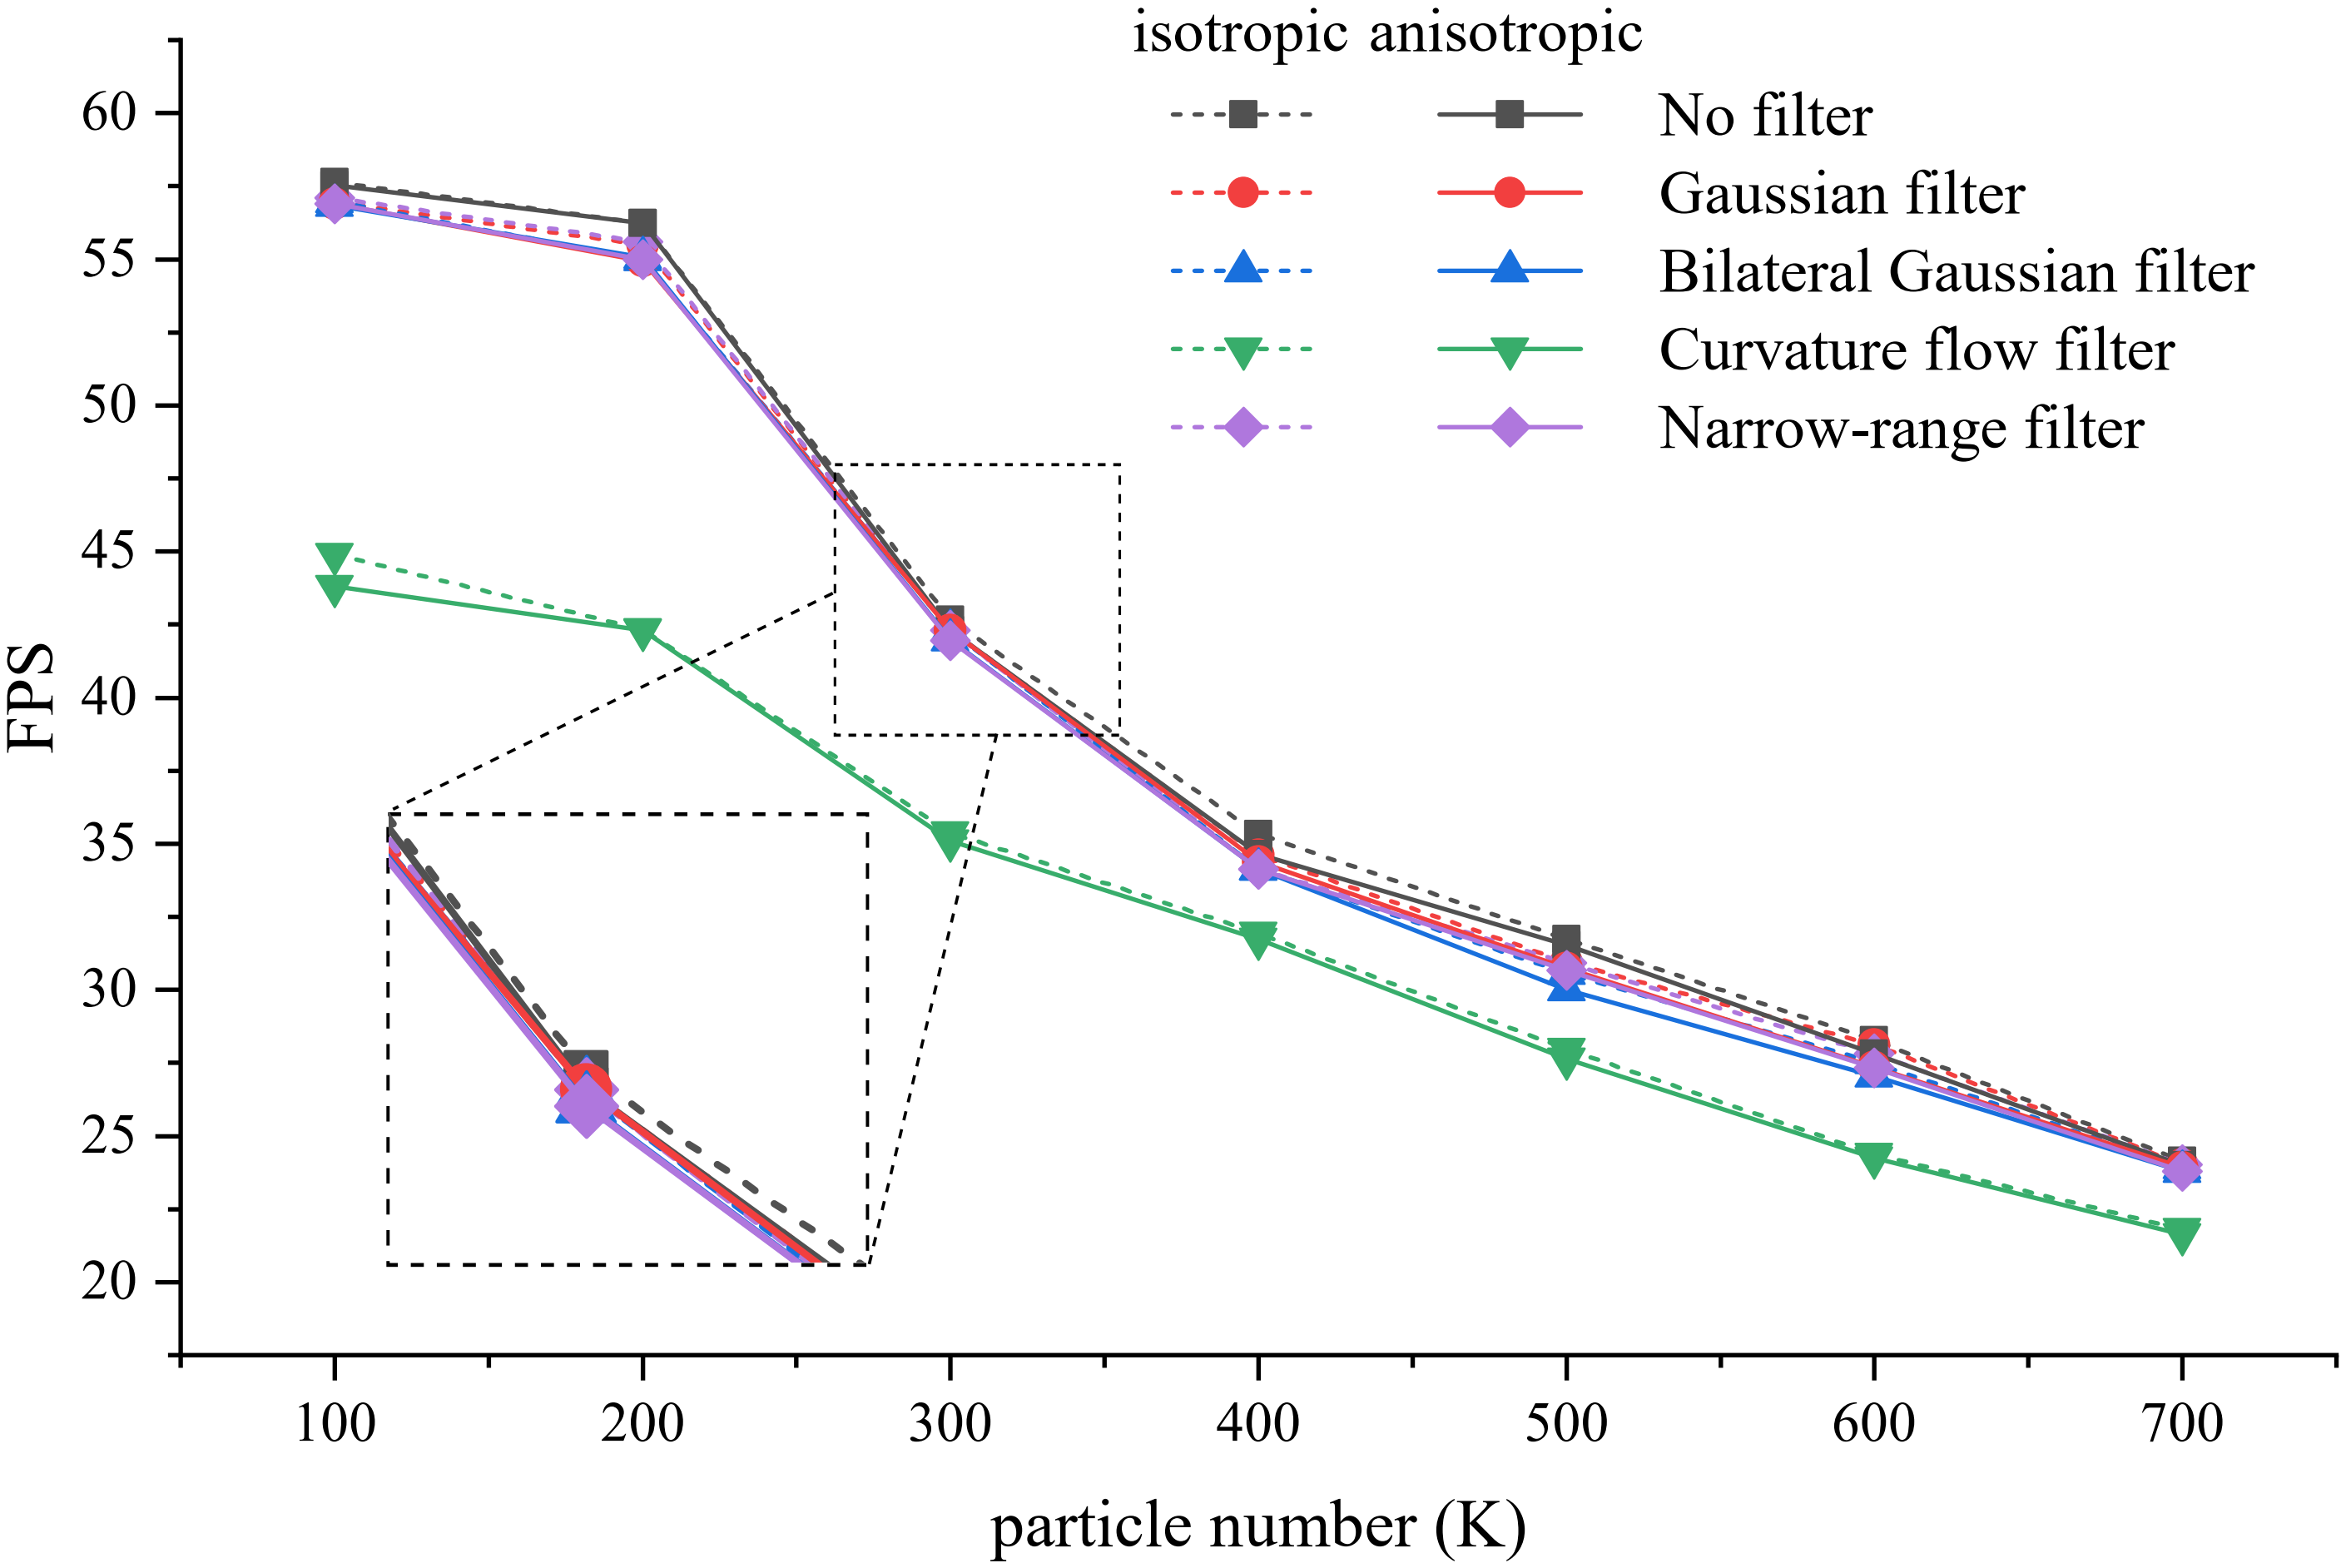
\includegraphics[width=\linewidth]{figs/FPS.png}
    \DIFaddendFL \caption{Frame rate comparison of different algorithms.}
    \label{fig:figure8}
\end{figure}

\section{Conclusion}
We propose an anisotropic real-time surface rendering scheme based on the screen space approach. The method uses WPCA to determine an anisotropic transform for particle point sprites, solving the problem of jagged edges and uneven surfaces of the fluid in traditional screen space rendering. We also compare the rendering effect and efficiency of various popular smoothing filters by experiments. It is concluded that the narrow-range filter is the preferred method for screen space rendering because it can obtain a better surface effect and maintain an acceptable frame rate. In the future, we will study the screen-space rendering of complex phenomena, such as the real-time visualization of multiphase fluid mixing, through the screen-space mapping of material type information.


\section*{Acknowledgments}
Acknowledgments should be inserted at the end of the paper, before the
references, not as a footnote to the title. Use the unnumbered
Acknowledgements Head style for the Acknowledgments heading.


\bibliographystyle{cag-num-names}
\bibliography{refs}


%%Vancouver style references.

\end{document}

%%
